\documentclass[svgnames,11pt]{beamer}
\input{/home/tof/Documents/Cozy/latex-include/preambule_commun.tex}
\input{/home/tof/Documents/Cozy/latex-include/preambule_beamer.tex}
%\usepackage{pgfpages} \setbeameroption{show notes on second screen=left}
\author[]{Christophe Viroulaud}
\title{Chiffrement symétrique}
\date{\framebox{\textbf{Archi 20}}}
%\logo{}
\institute{Terminale - NSI}

\begin{document}
\begin{frame}
    \titlepage
\end{frame}
\begin{frame}
    \frametitle{}

    La communication sur internet est organisée en couches.
    \begin{center}
        \begin{tabular}{|c|}
            \hline
            Couche application (Navigateur) \\
            \hline
            Couche TCP (Transport)          \\
            \hline
            Couche IP (Internet)            \\
            \hline
            Couche réseau (Matérielle)      \\
            \hline
        \end{tabular}
        \captionof{table}{Protocole TCP/IP}
    \end{center}

\end{frame}
\begin{frame}
    \frametitle{}
    \begin{center}
        \centering
        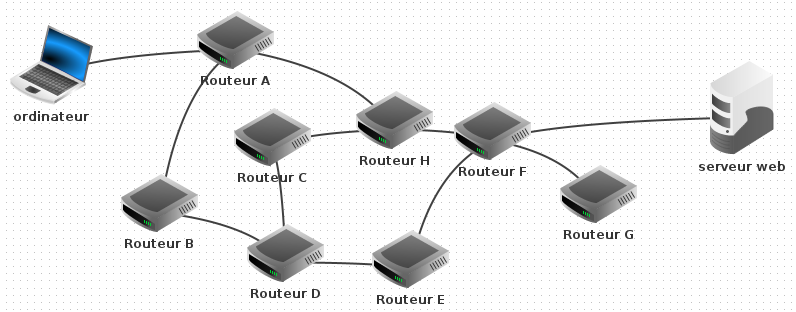
\includegraphics[width=8cm]{ressources/serveur-web.png}
        \captionof{figure}{\centering Les paquets IP transitent sur le réseau internet en circulant de routeurs en routeurs.}
        \label{IMG}
    \end{center}
    En théorie, rien n'interdit à un routeur d'inspecter un paquet et donc d'en connaître son contenu.
    \begin{framed}
        \centering Comment chiffrer le contenu des communications?
    \end{framed}
\end{frame}
\section{Chiffrement symétrique}
\begin{frame}
    \frametitle{Chiffrement symétrique}

    \begin{center}
        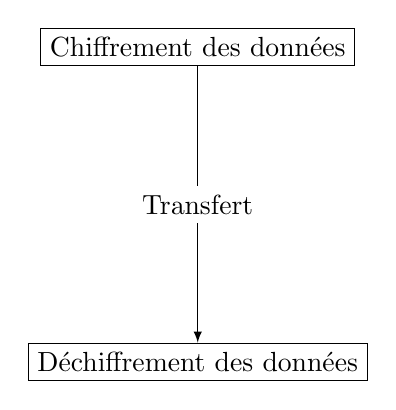
\begin{tikzpicture}
            \node[draw] (A) at (0,0) {Chiffrement des données};
            \node[draw] (B) at (0,-4) {Déchiffrement des données};
            \draw[->,>=latex] (A) -- (B) node[midway, fill=white] {Transfert};
        \end{tikzpicture}
    \end{center}

\end{frame}
\begin{frame}
    \frametitle{}

    \begin{itemize}
        \item<1-> La source utilise une \emph{fonction de chiffrement} pour coder un message \textbf{\texttt{m}} avec une clé de chiffrement \textbf{\texttt{k}}. La fonction produit en sortie un message chiffré \textbf{\texttt{s}}.
              \begin{center}
                  \textbf{\texttt{chiffrement(m, k) $\rightarrow$ s}}
              \end{center}
        \item<2-> Le destinataire utilise une \emph{fonction de déchiffrement} pour décoder le message \textbf{\texttt{s}} avec la clé de chiffrement \textbf{\texttt{k}}. La fonction produit en sortie le message clair \textbf{\texttt{m}}.
              \begin{center}
                  \textbf{\texttt{déchiffrement(s, k) $\rightarrow$ m}}
              \end{center}
    \end{itemize}

\end{frame}
\begin{frame}
    \frametitle{}

    \begin{aretenir}[]
        Dans un chiffrement symétrique on utilise la même clé pour chiffrer et déchiffrer le message.
        \end{aretenir}

\end{frame}
\section{Chiffrement de César}
\subsection{Algorithme}
\begin{frame}
    \frametitle{Chiffrement de César}

    Le chiffrement de César utilise un décalage alphabétique comme clé de chiffrement. Par exemple, avec la clé \textbf{\texttt{+2}}:
    \begin{itemize}
        \item A devient C
        \item B devient D
        \item \dots
        \item Z devient B
    \end{itemize}

\end{frame}
\begin{frame}[fragile]
    \frametitle{}
    
    \begin{activite}
        Écrire la fonction \textbf{\texttt{chiffrement(message: str, cle: int) $\rightarrow$ str}} qui code \textbf{\texttt{message}}. \\
        On n'utilisera que des caractères majuscules ASCII dans le message et on supprimera les espaces.     Dans un premier temps, on ne s'occupera pas du \emph{débordement de l'alphabet}. Ainsi l'appel
\begin{center}
\begin{lstlisting}[language=Python , basicstyle=\ttfamily\small, xleftmargin=2em, xrightmargin=2em]
>>> chiffrement("Z", 1)
\end{lstlisting}
\end{center}
renverra le caractère \textbf{\texttt{[}} situé à la 91° position du code ASCII.
    \end{activite}

\end{frame}
\begin{frame}[fragile]
    \frametitle{Correction}

\begin{center}
\begin{lstlisting}[language=Python , basicstyle=\ttfamily\small, xleftmargin=0.2em, xrightmargin=0em]
def chiffrement(message: str, cle: int) -> str:
    sortie = ""
    for lettre in message:
        # code ASCII de la lettre chiffrée
        code = ord(lettre) + cle
        # ajout
        sortie = sortie+chr(code)
    return sortie
\end{lstlisting}
\end{center}

\end{frame}
\begin{frame}[fragile]
    \frametitle{}

    \begin{activite}
    Modifier la fonction pour que l'appel
\begin{center}
\begin{lstlisting}[language=Python , basicstyle=\ttfamily\small, xleftmargin=2em, xrightmargin=2em]
>>> chiffrement("Z", 1)
\end{lstlisting}
\end{center}
renvoie la lettre \textbf{\texttt{A}}
    \end{activite}

\end{frame}
\begin{frame}[fragile]
    \frametitle{Correction}

\begin{center}
\begin{lstlisting}[language=Python , basicstyle=\ttfamily\small, xleftmargin=0.2em, xrightmargin=0em]
def chiffrement(message: str, cle: int) -> str:
    sortie = ""
    for lettre in message:
        # code ASCII de la lettre chiffrée
        code = ord(lettre) + cle
        # ajustement du code ASCII
        if code > ord("Z"):
            code = code-26
        # ajout
        sortie = sortie+chr(code)
    return sortie
\end{lstlisting}
\end{center}

\end{frame}
\begin{frame}
    \frametitle{}

    \begin{activite}
    Écrire la fonction \textbf{\texttt{dechiffrement(secret: str, cle: int) $\rightarrow$ str}} qui déchiffre \textbf{\texttt{secret}} en prenant en compte le \emph{débordement de l'alphabet}.
    \end{activite}

\end{frame}
\begin{frame}[fragile]
    \frametitle{Correction}

\begin{center}
\begin{lstlisting}[language=Python , basicstyle=\ttfamily\small, xleftmargin=0.2em, xrightmargin=0em]
def dechiffrement(secret: str, cle: int) -> str:
    sortie = ""
    for lettre in secret:
        # code ASCII de la lettre chiffrée
        code = ord(lettre) - cle
        # ajustement du code ASCII
        if code < ord("A"):
            code = code+26
        # ajout
        sortie = sortie+chr(code)
    return sortie

\end{lstlisting}
\begin{lstlisting}[language=Python , basicstyle=\ttfamily\small, xleftmargin=0.2em, xrightmargin=0em]
>>> secret = chiffrement("NSI",15) # CHX
>>> dechiffrement(secret, 15) # NSI
\end{lstlisting}
\end{center}

\end{frame}
\begin{frame}[fragile]
    \frametitle{}

    \begin{aretenir}[Remarque]
        Si la clé vaut \textbf{\texttt{13}}, la fonction de chiffrement permet également de déchiffrer.
        \end{aretenir}
\begin{center}
\begin{lstlisting}[language=Python , basicstyle=\ttfamily\small, xleftmargin=0.2em, xrightmargin=0em]
>>> chiffrement("NSI", 13) # AFV
>>> chiffrement("AFV", 13) # NSI
\end{lstlisting}
\end{center}

\end{frame}
\subsection{Un chiffrement faible}
\begin{frame}
    \frametitle{Un chiffrement faible}

    \begin{itemize}
        \item<1-> Le chiffrement de César n'offre que 25 clés.
        \item<2->La fréquence d'apparition des lettres est une méthode simple à mettre en place pour décrypter un message.
        \begin{center}
        \centering
        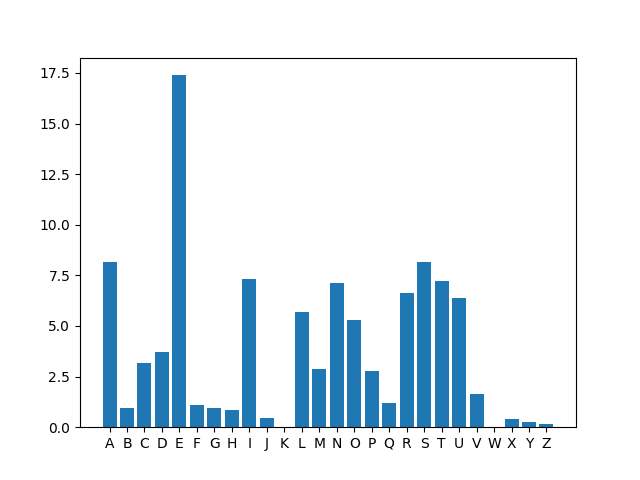
\includegraphics[width=7cm]{ressources/frequence-apparition.png}
        \captionof{figure}{Fréquences d'apparition des lettres}
        \label{IMG}
        \end{center}
    \end{itemize}

\end{frame}
\section{Chiffrement polyalphabétique}
\subsection{Principe}
\begin{frame}
    \frametitle{Chiffrement polyalphabétique - Principe}
Il consiste à:
    \begin{itemize}
        \item utiliser une clé de chiffrement composée de plusieurs lettres,
        \item recopier la clé de façon à obtenir une chaîne de la longueur du message.
    \end{itemize}
\begin{center}
    \begin{tabular}{*{5}{c}}
        B&R&A&V&O\\
        N&S&I&N&S\\
    \end{tabular}
\end{center}


\end{frame}
\begin{frame}
    \frametitle{}
    \begin{center}
        \begin{aretenir}[Remarques:]
            \begin{itemize}
                \item<1-> Une même lettre ne sera plus forcément codée par le même symbole.
                \item<2-> Une clé de la même taille que le message garantit une protection sûre (téléphone rouge). 
                \item<3-> Cette méthode est utilisée dans le code de Vigenère ou la machine Énigma.
            \end{itemize}
        \end{aretenir}
        \end{center}
    

\end{frame}
\subsection{Porte XOR}
\begin{frame}
    \frametitle{Porte XOR}

    \begin{aretenir}[]
    La porte XOR est réversible:
    $$\mbox{Si }A\oplus B = C \mbox{ alors } A\oplus C=B \mbox{ et }B\oplus C=A$$
    \end{aretenir}

\end{frame}
\begin{frame}
    \frametitle{}

    \begin{center}
        \begin{tabular}{*{5}{c}}
            B&R&A&V&O\\
            66&82&65&86&79\\
            N&S&I&N&S\\
            78&83&73&78&83\\
        \end{tabular}
        \captionof{table}{Conversion en ASCII}
    \end{center}

\end{frame}
\begin{frame}
    \frametitle{}

    \begin{center}
        \begin{tabular}{*{5}{c}}
            B&R&A&V&O\\
    
            66&82&65&86&79\\
            1000010&1010010&1000001&1010110&1001111\\
            N&S&I&N&S\\
    
            78&83&73&78&83\\
            1001110&1010011&1001001&1001110&1010011\\
        \end{tabular}
        \captionof{table}{Conversion en binaire}
    \end{center}

\end{frame}
\begin{frame}
    \frametitle{}

    \begin{center}
        \begin{tabular}{*{6}{c}}
            Message&1000010&1010010&1000001&1010110&1001111\\
            $\oplus$&1001110&1010011&1001001&1001110&1010011\\
            \hline
            Chiffré&0001100&0000001&0001000&0011000&0011100\\
        \end{tabular}
        \captionof{table}{Application de la porte XOR}
    \end{center}
\end{frame}
\begin{frame}
    \frametitle{}
    \begin{aretenir}[Remarque]
        Le message chiffré est envoyé, puis une application de la porte XOR avec la même clé permet de retrouver le message d'origine.
        \end{aretenir}
    \begin{center}
        \begin{tabular}{*{6}{c}}
            Chiffré&0001100&0000001&0001000&0011000&0011100\\
            
            $\oplus$&1001110&1010011&1001001&1001110&1010011\\
            \hline
            Message&1000010&1010010&1000001&1010110&1001111\\
        \end{tabular}
        \captionof{table}{Application de la porte XOR}
    \end{center}

\end{frame}
\section{Utilisations}
\begin{frame}
    \frametitle{Utilisations}

    La fonction \textbf{\texttt{xor}} est implémentée dans les processeurs: il est possible de chiffrer en temps réel: 
    \begin{itemize}
        \item chiffrement d'un disque dur,
        \item chiffrement des données d'un smartphone.
    \end{itemize}

\end{frame}
\begin{frame}
    \frametitle{}

    La méthode est utilisée dans plusieurs algorithmes de chiffrement:
    \begin{itemize}
        \item<1-> algorithme DES (Data Encryption Standard) \begin{itemize}
            \item obsolète à cause d'une clé maximale de 56 bits ($2^{56}$ possibilités),
            \item lenteur pendant le chiffrage.
        \end{itemize}
        \item<2-> algorithme AES (Advanced Encryption Standard):
        \begin{itemize}
            \item utilise une clé 128 bits,
            \item choisi par l'institut de standardisation américain NIST (National Institute of Standards and Technology) en décembre 2001.
        \end{itemize}
        \item<3-> Chacha20: 
        \begin{itemize}
            \item date de 2008,
            \item améliore les performances d'un autre algorithme (Salsa20),
            \item 20 étapes de mélange.
        \end{itemize}
    \end{itemize}

\end{frame}
\end{document}